% Scalar regression on UCI datasets. \input this file from the main report.
% It needs amsmath, amssymb, graphicx, booktabs; the figures sit next to the .tex files.
% It refers to eq:score and eq:hcm-loss, which are defined in the main file.

\section{Scalar Regression on UCI Datasets}
\label{sec:uci}

This section answers Q3 (what the score measures for a scalar target, and how to obtain
intervals with a stated coverage) and the regression part of Q4 (training sensitivity). The
HCM paper evaluates regression on six UCI datasets \citep{dua2017uci,hernandez2015pbp} and reports one
result: the score $u$ grows when Gaussian noise is added to the test inputs. The official
repository has no UCI code, so the implementation is ours.

\subsection{Setup}
\label{sec:uci-setup}

We use the paper's six datasets (wine, concrete, energy, kin8nm, power, yacht) and its
protocol (Appendix~A.1): a random 80/10/10 split, an MLP with three hidden layers of 20
units, Adam with weight decay $10^{-4}$, 200 epochs, and test inputs perturbed by
$\mathcal{N}(0,\sigma^2 I)$ with $\sigma\in\{0,\dots,5\}$. The paper does not state the
batch size or the input scaling; we use batch size 64 and standardized inputs. The baselines share the trunk: a plain MLP, a Deep Ensemble of five
Gaussian-likelihood networks \citep{lakshminarayanan2017simple}, and MC Dropout with rate
0.1 and 50 passes \citep{gal2016dropout}. Results are means over 20 seeds (5 for sweeps).

Following Section~2.2 of the paper, a scalar target $t$ is embedded as $y=(t,t)$, so that
\begin{equation}
  R=\lVert y\rVert_2=\sqrt{2}\,\lvert t\rvert,\qquad
  d=\frac{y}{R}=\operatorname{sign}(t)\,\frac{(1,1)}{\sqrt{2}} .
  \label{eq:scalar}
\end{equation}
The network has a direction head $\hat d\in\mathbb{R}^2$ and a magnitude head
$\hat R\in\mathbb{R}$ and minimizes
\begin{equation}
  \mathcal{L}=\operatorname{MSE}(\hat R\,d,\;y)+\operatorname{MSE}(R\,\hat d,\;y)
  +\lambda_{\text{norm}}\bigl(\lVert\hat d\rVert_2-1\bigr)^2 ,
  \label{eq:loss}
\end{equation}
the squared-loss instance of Eq.~\eqref{eq:hcm-loss}, with $\lambda_{\text{norm}}=0$ unless
stated, as the paper recommends. The prediction is the mean of the two components of
$\hat R\hat d$ (the paper does not specify this). The score is Eq.~\eqref{eq:score} with
$\lvert\hat R\rvert$ in place of $\hat R$, because the magnitude head is an unconstrained
linear output.

\subsection{Reproduction and the learning rate}
\label{sec:uci-lr}

With the paper's stated setting (raw targets, learning rate $10^{-4}$), HCM does not finish
training on three datasets: its test RMSE is $1.67$, $1.69$ and $1.17$ times the standard
deviation of the targets on concrete, energy and yacht, worse than predicting the training
mean. The unstated batch size explains part of the gap to the paper: with batch size 1 our
validation MAE on concrete falls from $22.2$ to $4.94$ (paper: $4.31$). We therefore train
every method, including the baselines, with standardized targets and learning rate
$10^{-3}$, so that no method is undertrained. The RMSE of HCM is then still above that of
the plain MLP on all six datasets, by 2\% (power, wine) to 68\% (energy) (Wilcoxon
signed-rank test over seeds, $p\le 0.017$ on each).

\subsection{What the score measures for a scalar target}
\label{sec:uci-measure}

Eq.~\eqref{eq:scalar} shows that the direction carries one bit: the sign of $t$. With
$\lambda_{\text{norm}}=0$, the two squared-error terms of Eq.~\eqref{eq:loss} are minimized
pointwise by $\hat R^\star(x)=\mathbb{E}[R\mid x]$ and
$\hat d^\star(x)=\mathbb{E}[R^2 d\mid x]\,/\,\mathbb{E}[R^2\mid x]$, hence
\begin{equation}
\begin{split}
\lVert\hat d^\star(x)\rVert_2
&=\frac{\bigl\lvert\mathbb{E}\bigl[t\,\lvert t\rvert \mid x\bigr]\bigr\rvert}
        {\mathbb{E}\bigl[t^2\mid x\bigr]}\;\le\;1, \\
u^\star(x)
&=\sqrt{2}\;\mathbb{E}\bigl[\lvert t\rvert\mid x\bigr]
  \bigl(1-\lVert\hat d^\star(x)\rVert_2\bigr).
\end{split}
\label{eq:ustar}
\end{equation}
The norm equals 1 exactly when the sign of $t$ is certain given $x$. Three predictions
follow, and the experiments confirm each.

\begin{figure}[t]
  \centering
  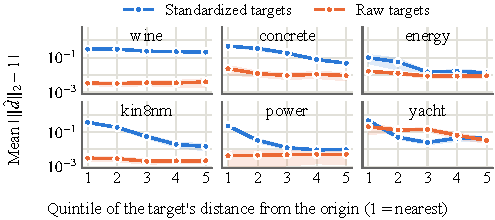
\includegraphics[width=\linewidth]{fig_origin}
  \caption{Violation of the unit-norm constraint by quintile of the target's distance from
  the origin (band: $\pm1$ std over 5 seeds). With standardized targets the violation is
  concentrated near the origin, which is the training mean.}
  \label{fig:origin}
\end{figure}

\emph{(i) With targets of one sign, $u$ carries no information on clean data.} All six raw
UCI targets are positive, so $d$ is constant and $u^\star=0$. In agreement, the mean
$\lVert\hat d\rVert_2$ with raw targets is within $0.015$ of 1 on five datasets.

\emph{(ii) After centering, $u$ marks targets near the mean, not large errors.}
Standardizing makes the sign uncertain near zero. The mean norm drops to between $0.78$ and
$0.98$, and the violation is 10 to 27 times larger in the quintile of targets nearest the
origin than in the farthest one on concrete, kin8nm and power (Figure~\ref{fig:origin}).
The score does not rank errors: on wine, kin8nm and power its Spearman correlation with the
absolute error is at most $0.06$ in absolute value.

\emph{(iii) The HCM prediction is not the conditional mean.} For
$t\mid x\sim\mathcal{N}(\mu,s^2)$ with $\lvert\mu\rvert\ll s$ the prediction is $(4/\pi)\mu$,
a 27\% overshoot, which is consistent with the accuracy cost of
Section~\ref{sec:uci-lr}.

\paragraph{Scale and noisy inputs.} Eq.~\eqref{eq:ustar} is equivariant to rescaling $t$,
but training at a fixed learning rate is not: multiplying the kin8nm target by $0.1$ lowers
the AUROC for detecting noisy inputs ($\sigma=5$) from $0.97$ to $0.35$. The paper's claim
about perturbed inputs does reproduce: with standardized targets the AUROC is $0.86$ to
$0.99$ at $\sigma=5$. The score detects unusual inputs; it does not predict the error.

\subsection{From scores to calibrated intervals}
\label{sec:uci-intervals}

The paper calibrates $u$ with one temperature $T$, fitted so that the coverage of
$\hat y\pm kTu$ for $k=1,2,3$ is closest to $68/95/99.7\%$. This gives no guarantee, and
the paper's own depth-estimation results miss the two higher levels ($0.88$ and $0.92$
against $0.95$ and $0.997$; its Table~3). We replace it with split conformal prediction
\citep{vovk2005algorithmic,angelopoulos2021gentle}. For a nominal coverage $p$ and a width
function $s(x)>0$, the interval is $\hat y(x)\pm q\,s(x)$, where $q$ is the
$\lceil (n+1)p\rceil$-th smallest value of $\lvert y_i-\hat y_i\rvert/s(x_i)$ over the $n$
validation points. Coverage is at least $p$ on exchangeable test data for any $s$. We
compare three width functions for HCM: \textbf{constant}, $s(x)=1$; \textbf{scaled},
$s(x)=u(x)$, the analogue of the paper's rule; and \textbf{floored} (ours),
$s(x)=\max\bigl(1,\,u(x)/u_{95}\bigr)$, where $u_{95}$ is the 95th percentile of $u$ on the
training set. The floored interval keeps a constant width in the usual range of $u$, where
$u$ does not rank errors, and widens only when $u$ is unusually large. IS denotes the
interval score of \citet{gneiting2007strictly}.

\begin{table}[t]
  \centering
  \small
  \setlength{\tabcolsep}{1mm}
  \begin{tabular}{@{}lcccccc@{}}
    \toprule
    & \multicolumn{3}{c}{clean test} & \multicolumn{2}{c}{$\sigma=1$} & $\sigma=5$ \\
    \cmidrule(lr){2-4}\cmidrule(lr){5-6}\cmidrule(l){7-7}
    Method & cov. & width & IS & cov. & IS & IS \\
    \midrule
    HCM temp.\ (paper)         & 0.845 & 2.87 & 3.46 & 0.752 & 15.8 & 256 \\
    HCM constant               & 0.896 & 1.01 & 1.40 & 0.359 & 16.6 & 217 \\
    HCM scaled by $u$          & 0.902 & 4.46 & 4.85 & 0.828 & 22.5 & 417 \\
    \textbf{HCM floored (ours)} & \textbf{0.893} & \textbf{1.01} & \textbf{1.39} & \textbf{0.485} & \textbf{10.2} & \textbf{56.0} \\
    \midrule
    MCD Gaussian               & 0.704 & 0.59 & 2.30 & 0.367 & 10.1 & 38.3 \\
    MCD conformal              & 0.900 & 1.16 & 1.49 & 0.539 & 7.8  & 30.9 \\
    DE Gaussian                & 0.925 & 0.91 & 1.18 & 0.456 & 9.9  & 42.3 \\
    DE conformal               & 0.905 & 0.89 & 1.18 & 0.427 & 10.3 & 42.6 \\
    \bottomrule
  \end{tabular}
  \caption{Prediction intervals at nominal coverage $0.90$ (six datasets, 20 seeds). Width
  and interval score (IS, lower is better) are in units of std($y$). Temp.\ is the paper's
  temperature rule; constant, scaled and floored are conformal. MCD: MC Dropout; DE: Deep
  Ensemble.}
  \label{tab:intervals}
\end{table}

Table~\ref{tab:intervals} supports four conclusions.
\emph{(1) Conformal calibration repairs the paper's under-coverage.} The temperature rule
covers $84.5\%$ at a nominal $90\%$. Every conformal variant is within about one point of
$90\%$ on clean data, and the constant and floored intervals are about a third as wide.
\emph{(2) Scaling the width by $u$ is harmful.} Because $u$ is close to zero for many clean
inputs, the intervals are $4.4$ times wider.
\emph{(3) The floored rule keeps the benefit of $u$ without that cost.} On clean data it
matches the constant interval ($1.39$ against $1.40$). Under input noise it lowers the
interval score from $16.6$ to $10.2$ at $\sigma=1$ and from $217$ to $56$ at $\sigma=5$.
\emph{(4) HCM does not beat the sampling baselines, but it is cheaper.} The Deep Ensemble
has the best clean interval score ($1.18$). At $\sigma=1$ floored HCM equals it ($10.2$
against $10.3$) with one network instead of five; at $\sigma=5$ it is behind both
baselines. Under noise no method keeps the guarantee: coverage at $\sigma=1$ falls to
between $0.36$ and $0.54$, except for the two very wide HCM intervals.

\subsection{Our Improvements: a Prediction Head and Residual-Origin HCM}
\label{sec:uci-fix}

Section~\ref{sec:uci-measure} found two causes of the problems above: the HCM prediction is
not the conditional mean, and the origin of the decomposition is arbitrary. Each suggests
one change; both keep the loss of Eq.~\eqref{eq:loss}.

\paragraph{A separate prediction head.} We add a linear head $f(x)$ trained with the plain
MSE and use it as the prediction; the HCM heads only produce the score. When the HCM heads
are \emph{detached} (they read the trunk features but send no gradient back) or have their
\emph{own} trunk, the accuracy cost disappears: the test RMSE is $1.003$ and $1.005$ times
that of the plain MLP (Wilcoxon, $p\ge 0.097$ on every dataset). With a shared trunk the
ratio is $1.09$ (Figure~\ref{fig:fix}, top left).

\paragraph{Residual-origin HCM.} We apply the decomposition to the standardized residual
$r=(t-f(x))/s$ instead of the target, where $s$ is a running root-mean-square of the
training residuals and no gradient flows into $f$. Eq.~\eqref{eq:ustar} holds with $r$ in place of $t$: if the sign of the residual
cannot be predicted from $x$, then $\lVert\hat d^\star\rVert_2=0$ and
$\hat R^\star=\sqrt2\,\mathbb{E}[\lvert r\rvert\mid x]$, the expected absolute error up to a
constant. We therefore use $R_r=s\,\lvert\hat R\rvert$ as the score.

On clean data the new score does what $u$ could not (Table~\ref{tab:fix}). Its Spearman
correlation with the absolute error is $0.24$ against $0.15$ for $u$. A conformal interval
with width proportional to $R_r$ has an interval score of $1.27$, against $1.39$ for
floored HCM. The cost is that $R_r$ does not
detect unusual inputs: its AUROC at $\sigma=5$ is $0.67$ against $0.94$ for $u$. The two
scores are complementary: $R_r$ ranks errors on data like the training data, and the
target-origin score, written $u_t$, flags inputs unlike it.

\begin{table}[t]
  \centering
  \small
  \setlength{\tabcolsep}{1mm}
  \begin{tabular}{@{}lcccccc@{}}
    \toprule
    & & & & clean & $\sigma=1$ & $\sigma=5$ \\
    Width function & RMSE & $\rho$ & AUROC & IS & IS & IS \\
    \midrule
    HCM, floored $u$           & 1.196 & 0.15 & 0.94 & 1.39 & 10.2 & 56.0 \\
    \midrule
    \multicolumn{7}{@{}l}{\emph{Prediction head, detached HCM heads (one trunk)}} \\
    floored $u_t$              & 1.003 & 0.13 & 0.86 & 1.32 & 11.7 & 43.1 \\
    $R_r$                      & 1.003 & 0.24 & 0.67 & 1.27 & 13.7 & 74.0 \\
    both, product rule         & 1.003 & 0.24 & 0.84 & 1.27 & 11.5 & 63.9 \\
    \textbf{both, max rule}    & \textbf{1.003} & \textbf{0.23} & \textbf{0.89} & \textbf{1.27} & \textbf{11.8} & \textbf{43.5} \\
    \midrule
    \multicolumn{7}{@{}l}{\emph{Prediction head, HCM heads with their own trunks}} \\
    both, max rule             & 1.005 & 0.28 & 0.94 & 1.27 & 10.7 & 50.2 \\
    \midrule
    Deep Ensemble              & 1.244 & 0.42 & 0.98 & 1.18 & 10.2 & 42.6 \\
    MC Dropout                 & 1.431 & 0.15 & 0.97 & 1.49 & 7.8  & 30.9 \\
    \bottomrule
  \end{tabular}
  \caption{Our improvements (six datasets, 20 seeds, conformal intervals at nominal coverage
  $0.90$; clean coverage $0.893$ to $0.905$). RMSE is relative to the plain MLP; $\rho$ is
  the Spearman correlation of the width with the absolute error; AUROC is for noisy inputs
  at $\sigma=5$. Bold: our proposed variant.}
  \label{tab:fix}
\end{table}

\begin{figure}[t]
  \centering
  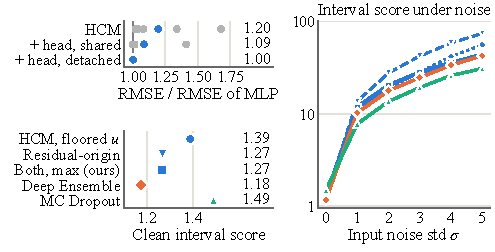
\includegraphics[width=\linewidth]{fig_changes}
  \caption{Top left: test RMSE relative to the plain MLP (gray: single datasets).
  Bottom left: clean interval score. Right: interval score under input noise (same
  markers). Six datasets, 20 seeds, detached heads.}
  \label{fig:fix}
\end{figure}

\paragraph{Using both scores.} With detached heads, a target-origin pair and a
residual-origin pair can share one trunk and one forward pass. We compare two width functions, with $u_{95}$ as in
Section~\ref{sec:uci-intervals} and $\bar R_r$ the training mean of $R_r$:
\begin{align*}
\text{product:}\quad s(x) &= R_r(x)\,\max\!\Bigl(1,\frac{u_t(x)}{u_{95}}\Bigr),\\
\text{max:}\quad s(x) &= \max\!\Bigl(\frac{R_r(x)}{\bar R_r},\,\frac{u_t(x)}{u_{95}}\Bigr).
\end{align*}
Both keep the clean-data gain ($1.27$). The product rule fails at $\sigma=5$ ($63.9$). The
max rule reaches $43.5$ at $\sigma=5$, better than floored HCM ($56.0$) and level with the
Deep Ensemble ($42.6$), but at $\sigma=1$ it is worse than floored HCM ($11.8$ against
$10.2$). Over five target preprocessings the interval score of $R_r$ ranges from $1.29$ to
$1.75$, against $3.57$ to $6.79$ for the original score. Residual-origin HCM is close to estimating the absolute residual for locally weighted
conformal intervals \citep{lei2018conformal}.

\paragraph{Norm penalty and warm-up (Q4).} With standardized targets, raising
$\lambda_{\text{norm}}$ from 0 to 5 moves the mean norm from $0.88$ to $0.99$, raises the
test error on 26 of 30 dataset--seed pairs, and raises the AUROC for noisy inputs from
$0.93$ to $0.97$ at $\sigma=5$. A warm-up of 5 or 20 epochs changes the normalized RMSE by
at most $0.01$ and the AUROC by at most $0.02$, so it is not needed here.

\paragraph{Limitations.}
\label{sec:uci-limits}
The network is a small MLP. The analysis assumes squared losses,
$\lambda_{\text{norm}}=0$ and clean inputs, so it does not explain why $u$ rises under
noise. The max rule was selected on the noisy test sets, so its results under noise are exploratory.
